\documentclass[10pt]{article}
\usepackage{listings}
\usepackage[utf8]{inputenc}
\usepackage[margin=1in]{geometry} 
\usepackage{amsmath,amsthm,amssymb, graphicx, multicol, array, caption, subcaption}
\usepackage{textcomp}
\usepackage{tikz}
 \lstset{language=Python}    
\newcommand{\N}{\mathbb{N}}
\newcommand{\Z}{\mathbb{Z}}
 \renewcommand{\qedsymbol}{}
 \renewcommand{\delta}{\partial}
\newenvironment{problem}[2][Partie]{\begin{trivlist}
\item[\hskip \labelsep {\bfseries #1}\hskip \labelsep {\bfseries #2.}]}{\end{trivlist}}
\begin{document}
 
\title{Carnet de Bord}
\author{R. Seguel, J.P. Soto, P. Cuello et M. Bataille}
\date{Avril, Mai et Juin 2016}
\maketitle
 \section{Réunion 1. 27/04}


{\bf Équations.}

On a déterminé
l'expression de l'équation horaire:
$$ z(t) = \frac{1}{2}gt^2+v_0\sin\alpha\times t+z_0$$

Où $v_0$ est la vitesse initiale, $z_0$ est la hauteur
initiale ($h$) et $\alpha$ est l'angle du lancer de la balle.

D'après cette expression, on a déduit l'équation de la
hauteur en fonction de la distance horizontale**:
$$ t=\frac{-g}{2v_0^2\cos^2\alpha}y^2+\tan\alpha\times y+h $$

{\bf Plans}

On a contacté un professeur aux E.U., Mr Lance, et ils nous
a envoyé les plans de son trébuchet (MURLIN).

Problème: Mr. Lance nous a dit qu'il faut réguler la
 longueur du bras et de la corde puisqu'ils sont pensés pour
 un trébuchet de 3m de hauteur et pour un projectile 4 fois plus léger.
 
 Potentielles solutions:
\begin{enumerate}
 \item On peut faire un prototype pour ensuite réaliser des expériences
 et on déduit les longueurs du bras et de la corde optimales
 pour le trébuchet à échelle réelle (2m). Mais, on prend tu temps
 et de ressources sur le prototype.
 \item  On peut faire une simulation, mais elle
 nécessite des outils mathématiques complexes. Mais, il faut comprendre ces outils mathématiques
 et ensuite les implementer, ce qui prend tu temps, mais pas
 de ressources (monétaires).
 \item  On fait directement le trébuchet à échelle
 réelle et on régule directement les longueurs du bras et de
 la corde sur ce trébuchet.
\end{enumerate}

\vspace{1cm}
\section{Réunion 2. 28/04}

{\bf Plans}
On a calculé la plupart des mesures pour un raccourcissement de 67\% comme Mr Lance nous le a indiqué.

Mais, lors de faire plusieurs calculs sur la hauteur avec un angle du lancer de $\alpha = 71$\textdegree, on remarque qu'on peut faire
un raccourcissement de 76\%. C'est, malgré tout, une différence de 10\% qui pourrait avoir un grand impact sur la distance
parcourue par la balle. Il faut donc faire une meilleure estimation pour le taux de raccourcissement trébuchet.
parcourue par la balle. D'ailleurs, si notre estimation de l'angle du lancer est érronée, et que l'angle vaut $\alpha = 45$\textdegree, la
hauteur, avec ce raccourcissement, serait de $1.68m$ alors qu'elle devriait être le plus proche de $2m$ possible.

En regardant la simulation faite par Mr. Lance, on observe que l'angle
du lancer est de $60$\textdegree. D'où le taux de raccourcissement serait
de 80\%.

\vspace{1cm}
\section{Vacances.}

Finalement, on a décidé de faire un raccourcissement de 80\% puisqu'il faudra raccourcir le bras et la corde de quelques centimètres du au poids du projectile. Les mesures calculées sont affichées sur la figure ci-dessous. 

\begin{figure}[h]
\centering
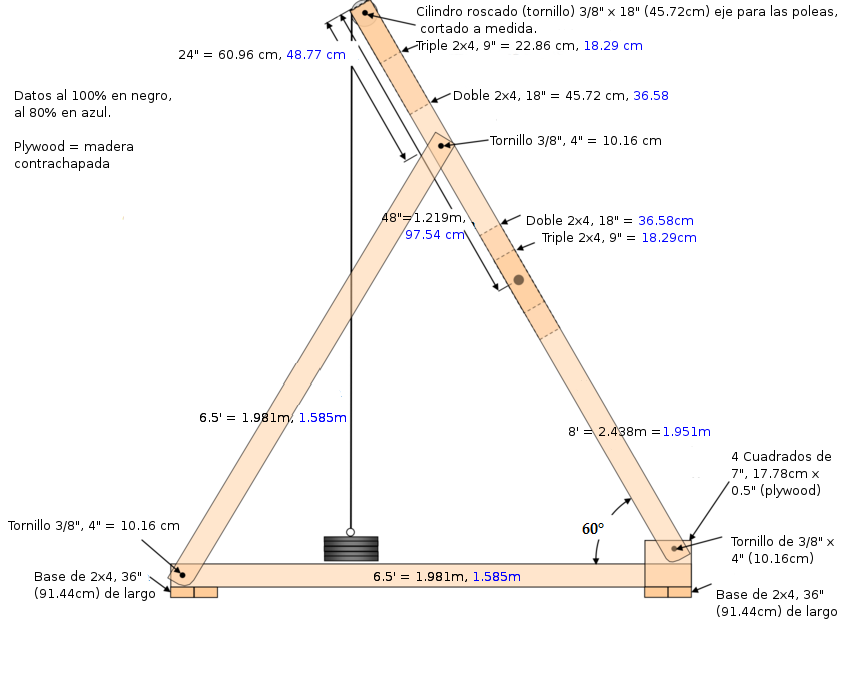
\includegraphics[width=0.7\textwidth]{medidas2.png}
\end{figure}

\section{Travail sur la simulation.}
Pour pouvoir étudier plus facilement les mécaniques du trébuchet, on commencera par diviser le problème en plusieurs parties, plus simples.

\subsection{Deux particules, une corde}

D'abord, on étudiera le mouvement d'une particule $B$ attachée à une autre particule $A$ par une corde de longueur $\ell$ lorsque la particule $A$ a une certaine vitesse $\vec{v}$. La configuration initiale est celle de la première figure.


\begin{figure}[!h]
\centering
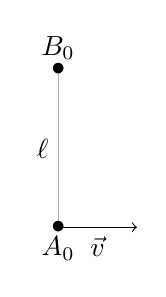
\begin{tikzpicture}
	\centering
	\draw[color=gray!60] (0,0) -- (0,2) ;
    \draw  [->] (0,0) -- (1,0);
   \draw (0.5,0) node[below] {$\vec{v}$} ;
   \draw (0,0) node[below] {$A_0$};
   \draw (0,0) node {$\bullet$} ;
   \draw (0,2) node {$\bullet$};
   \draw (0,2) node[above] {$B_0$};
   \draw (0,1) node[left] {$\ell$};
\end{tikzpicture}
\hspace{2cm}
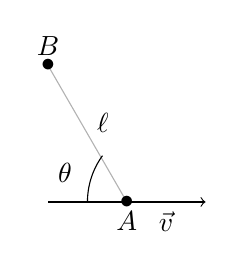
\begin{tikzpicture}
	\draw[color=gray!60] (1,0) -- (0,1.732) ;
    \draw  [->] (1,0) -- (2,0);
   \draw (1.5,0) node[below] {$\vec{v}$} ;
   \draw (1,0) node[below] {$A$};
   \draw (1,0) node {$\bullet$} ;
   \draw (0,1.732) node {$\bullet$};
   \draw (0,1.732) node[above] {$B$};
   \draw (0.5,1) node[right] {$\ell$};	
   \draw (0,0) -- (1,0);
   \draw (0.5,0) arc (180:144:1);
   \draw (60:0.43) node {$\theta$} ;
\end{tikzpicture}
\end{figure}
Dans un premier temps on étudiera cette situation en prennant $\vec{v}$ constant.

On utilisera des coordonnées cartésiennes telles que $A_0 = (0;0)$ et $B_0 = (0;2)$. On a:
\begin{align*}
y_A &= 0 \\
x_B &= x_A - \ell\cos{\theta}\\
y_B &= \ell\sin{\theta}
\end{align*}

On détermine l'expression de l'énergie cinétique,

\begin{align*}
T &= \frac{1}{2}m_A(\dot{x}_A ^2 + \dot{y}_A ^2) + \frac{1}{2}m_B(\dot{x}_B ^2 + \dot{y}_B ^2) \\
 &= \frac{1}{2}m_A\dot{x}_A ^2 + \frac{1}{2}m_B(\dot{x}_A+\dot{\theta}\ell\sin{\theta})^2 + \frac{1}{2}m_B(\dot{\theta}\ell\cos{\theta})^2 \\
 &= \frac{1}{2}m_A\dot{x}_A ^2 + \frac{1}{2}m_B\dot{x}_A ^2
 + \frac{1}{2}m_B \ell^2\dot{\theta}^2\sin^2{\theta} + m_B\dot{x}_A\ell\dot{\theta}\sin{\theta} 
 + \frac{1}{2}m_B\ell^2\dot{\theta}^2 \cos^2{\theta} \\
 &= \frac{1}{2}m_A\dot{x}_A ^2 + m_B\dot{x}_A\ell\dot{\theta}\sin{\theta}
 + \frac{1}{2}m_B \ell^2\dot{\theta}^2(\sin^2{\theta} + \cos^2{\theta}) \\
 &= \frac{1}{2}m_A\dot{x}_A ^2 + m_B\dot{x}_A\ell\dot{\theta}\sin{\theta}
 + \frac{1}{2}m_B \ell^2\dot{\theta}^2
\end{align*}

On détermine l'expression de l'énergie potentielle,

\begin{align*}
V &=m_Bgy_B \\
  &=m_Bg\ell\sin{\theta}
\end{align*}

On en déduit le lagrangien,
\begin{align*}
L &= T - V \\
 &= \frac{1}{2}m_A\dot{x_a}^2 + m_B\dot{x_a}\ell\dot{\theta}\sin{\theta}
 + \frac{1}{2}m_B \ell^2\dot{\theta}^2 -  m_Bg\ell\sin{\theta}
\end{align*}

D'ou on déduit,
\begin{align*}
 \frac{\delta L}{\delta\theta} &= m_B\dot{x}_A\ell\dot{\theta}\cos{\theta}-m_Bg\ell\cos{\theta} \\
 \frac{\delta L}{\delta \dot{\theta}} &= m_B\ell^2\dot{\theta} + m_B\dot{x}_A\ell\sin{\theta} \\
 \frac{d}{dt}\left(\frac{\delta L}{\delta \dot{\theta}}\right) &= m_B\ell^2\ddot{\theta}+m_B\dot{x_A}\ell\dot{\theta}\cos{\theta} 
\end{align*}

Or on sait que,
\begin{align*}
  \frac{\delta L}{\delta\theta} &= \frac{d}{dt}\left(\frac{\delta L}{\delta \dot{\theta}}\right) \\
  m_B\dot{x}_A\ell\dot{\theta}\cos{\theta}-m_Bg\ell\cos{\theta} &=  m_B\ell^2\ddot{\theta}+m_B\dot{x_A}\ell\dot{\theta}\cos{\theta}  \\
  \ddot{\theta} &= -\frac{g}{\ell}\cos{\theta}
\end{align*}

Pour les conditions initiales on a $\theta_0 = \frac{\pi}{2}$ d'où,
\begin{align*}
\ddot{\theta}_0 &= -\frac{g}{\ell}\cos{\theta_0}  \\
&= -\frac{g}{\ell}\cos{\frac{\pi}{2}} \\
&= 0
\end{align*}

Mais, si $\dot{\theta}_0 = 0$,  alors la vitesse angulaire ne changera pas (car $\ddot{\theta}_0 = 0$)et donc, la particule $B$ ne se déplacera pas par rapport à la particule $A$. On doit donc changer la configuration initiale, soit $\theta_0 \neq \frac{\pi}{2}$ (d'où $\ddot{\theta}_0 \neq 0$), soit $\dot{\theta}_0 \neq 0$ .

\subsection{Un disque, une particule et une corde}


Maintenant, on étudiera le mouvement d'une particule lorsqu'elle est attachée à un disque par une corde. La situation est celle de la figure ci-dessous. Pour conditions initiales, on prendra $\alpha = \beta = \frac12\pi$.
\begin{center}


\begin{tikzpicture}
\draw (0,0) circle (2);
\draw[->] (-3,0) -- (3,0);
\draw[->] (0,-3) -- (0,3);
\draw (45:2) node[above left] {$A$};
\draw (45:1.9) -- (45:2.1);
\draw (45:2) ++(2,0) node[below right] {$B$};
\draw (45:2) ++(2,0) node {$\bullet$};
\draw [dashed] (0:0) -- (45:2);
\draw (45:2) -- ++(2,0);
\draw (45:2) -- ++(0,1.5) -- ++(0,-4);
\draw[->] (-90:1) arc (-90:45:1);
\draw (-25:0.6) node {$\alpha$};
\draw[->] (45:2) ++(-90:1) arc (-90:0:1);
\draw (45:2) ++(-45:0.6) node {$\beta$};
\end{tikzpicture}
\end{center}
On notera $\ell_A$ le rayon du disque, $\ell_B$ la longueur de la corde et $m_B$ la masse de la particule $B$.

On détermine les coordonnées de la particule $B$:
\begin{align*}
x_B &= x_A + \ell_B\sin{\beta} \\
	&= \ell_A\sin{\alpha} + \ell_B\sin{\beta} \\
y_B &= y_A - \ell_B\cos{\beta} \\
	&= -\ell_A\cos{\alpha} - \ell_B\cos{\beta}
\end{align*}
D'où on déduit la vitesse de $B$, c'est à dire, la dérivée de sa position par rapport au temps:
\begin{align}
v_B(x) = \dot{x} &= \ell_A\dot{\alpha}\cos{\alpha} + \ell_B\dot{\beta}\cos{\beta} \\
v_B(y) = \dot{y} &= \ell_A\dot{\alpha}\sin{\alpha} + \ell_B\dot{\beta}\sin{\beta}
\end{align}
On utilisera l'équation de Langrange. Pour ce faire, on calculera l'expression de l'énergie cinétique $T$\footnote{Si on ne prend pas l'énergie cinétique rotationelle du disque, au moment de déterminer les équations différentielles, on divise par $\cos{(\alpha-\beta)}$ ce qui provoque des problèmes lorsque $\alpha \approx \beta$ et, si on fait une simulation avec un logiciel, on n'obtient aucun résultat cohérent} et l'énergie potentielle $V$:
\begin{align*}
T &= \frac12m_Bv_B^2 + \frac12I\omega^2 \\
	&= \frac12m_B\left(\ell_A^2\dot{\alpha}^2+\ell_B^2\dot{\beta}^2+ 2\ell_A\ell_B\dot{\alpha}\dot{\beta}\cos{(\alpha-\beta)}\right) + \frac12I\dot{\alpha}^2 \\
V &= m_Bgy_B \\
	&= -m_Bg\left(\ell_A\cos{\alpha} + \ell_B\cos{\beta}\right) \\
L &= T-V \\
 &= \frac12m_B\left(\ell_A^2\dot{\alpha}^2+\ell_B^2\dot{\beta}^2+ 2\ell_A\ell_B\dot{\alpha}\dot{\beta}\cos{(\alpha-\beta)}\right) + \frac12I\dot{\alpha}^2 + m_Bg\left(\ell_A\cos{\alpha} + \ell_B\cos{\beta}\right) \\
\end{align*}
On dérive le lagrangien pour chaque degré de liberté,
\begin{align*}
\frac{\partial L}{\partial \dot{\alpha}} &= m_B\ell_A^2\dot{\alpha}+m_B\ell_A\ell_B\dot{\beta}\cos{(\alpha-\beta)}+I\dot{\alpha} \\
\frac{d}{dt}\left(\frac{\partial L}{\partial \dot{\alpha}}\right) &= m_B\ell_A^2\ddot{\alpha} + m_B\ell_a\ell_B(\ddot{\beta}\cos{(\alpha-\beta)}-\dot{\beta}\sin{(\alpha-\beta)}(\dot{\alpha}-\dot{\beta}) ) + I\ddot{\alpha}\\
\frac{\partial L}{\partial \dot{\beta}} &= m_B\ell_B^2\dot{\beta}+m_B\ell_A\ell_B\dot{\alpha}\cos{(\alpha-\beta)} \\
\frac{d}{dt}\left(\frac{\partial L}{\partial \dot{\beta}}\right) &= m_B\ell_B^2\ddot{\beta} + m_B\ell_A\ell_B(\ddot{\alpha}\cos{(\alpha-\beta)}-\dot{\alpha}\sin{(\alpha-\beta)}(\dot{\alpha}-\dot{\beta})) \\
\frac{\partial L}{\partial \alpha} &= -m_B\ell_A\ell_B\dot{\alpha}\dot{\beta}\sin{(\alpha - \beta)} - m_Bg\ell_A\sin{\alpha} \\
\frac{\partial L}{\partial \beta} &= m_B\ell_A\ell_B\dot{\alpha}\dot{\beta}\sin{(\alpha-\beta)}-m_Bg\ell_B\sin{\beta}
\end{align*}
On en déduit les équations de Lagrange,
\begin{align}
 \frac{\partial L}{\partial \alpha} &= \frac{d}{dt}\left(\frac{\partial L}{\partial \dot{\alpha}}\right) \nonumber \\
 -m_B\ell_A\ell_B\dot{\alpha}\dot{\beta}\sin{(\alpha-\beta)}-m_Bg\ell_A\sin{\alpha} &= m_B\ell_A^2\ddot{\alpha}+m_B\ell_A\ell_B(\ddot{\beta}\cos{(\alpha-\beta)}-\dot{\beta}\sin{(\alpha-\beta)}(\dot{\alpha}-\dot{\beta}))+I\ddot{\alpha} \nonumber \\
 -m_Bg\ell_A\sin{\alpha} &= (I+m_b\ell_A^2)\ddot{\alpha} + m_B\ell_A\ell_B\ddot{\beta}\cos{(\alpha-\beta)} + m_B\ell_A\ell_B\dot{\beta}^2\sin{(\alpha-\beta)} \nonumber\\
 \left(\frac{I}{m_B}+\ell_A^2\right)\ddot{\alpha} + \ell_A\ell_B\ddot{\beta}\cos{(\alpha-\beta)} &= -g\ell_A\sin{\alpha}-\ell_A\ell_B\dot{\beta}^2\sin{(\alpha-\beta)}
 \\
  \frac{\partial L}{\partial \beta} &= \frac{d}{dt}\left(\frac{\partial L}{\partial \dot{\beta}}\right) \nonumber \\
  m_B\ell_A\ell_B\dot{\alpha}\dot{\beta}\sin{(\alpha-\beta)}-m_Bg\ell_A\sin{(\beta)} &= m_B\ell_B\ddot{\beta}+m_B\ell_A\ell_B\ddot{\alpha}\cos{(\alpha-\beta)}-m_B\ell_A\ell_B\dot{\alpha}\sin{(\alpha-\beta)}(\dot{\alpha}-\dot{\beta}) \nonumber \\
 -m_Bg\ell_B\sin{\beta} &=m_B\ell_B^2\ddot{\beta}+m_B\ell_A\ell_B\ddot{\alpha}\cos{(\alpha-\beta)}-m_B\ell_A\ell_B\dot{\alpha}^2\sin{(\alpha-\beta)} \nonumber \\
\ell_B^2\ddot{\beta} +\ell_A\ell_B\ddot{\alpha}\cos{(\alpha-\beta)} &= \ell_A\ell_B\dot{\alpha}^2\sin{(\alpha-\beta)} -g\ell_B\sin{\beta}
 \end{align}
 
 Pour l'implémentation de la simulation, il faut cŕeer une fonction telle que $$\frac{dx}{dt} = f(x) $$

On a ici, 
\begin{align*}
x = \begin{pmatrix}
\alpha \\ \beta \\ \dot{\alpha} \\ \dot{\beta} 
\end{pmatrix} && f(x) = \begin{pmatrix}
\dot{\alpha} \\ \dot{\beta} \\ \ddot{\alpha} \\ \ddot{\beta}
\end{pmatrix}
\end{align*} 

Or, on connaît déjà l'expression de $\dot{\alpha}$ et $\dot{\beta}$ en fonction de $x$ . Il faut donc déterminer l'expression de $\ddot{\alpha}$ et $\ddot{\beta}$ en fonction de $x$. D'après $(3)$ et $(4)$,

\begin{equation*}
\begin{pmatrix}
A & B \\ C & D
\end{pmatrix}
\begin{pmatrix}
\ddot{\alpha} \\ \ddot{\beta}
\end{pmatrix}
=
\begin{pmatrix}
E  \\ F
\end{pmatrix}
\end{equation*}


Avec,
\begin{tabular}{ccc}
$A = \frac{I}{m_B}+\ell_A^2$ & $B = \ell_A\ell_B\cos{(\alpha-\beta)}$ & $E =-g\ell_A\sin{\alpha} - \ell_A\ell_B\dot{\beta}^2\sin{(\alpha-\beta)}$ \\
$C = \ell_A\ell_B\cos{(\alpha-\beta)}$ & $D = \ell_B^2$ & $F=\ell_A\ell_B\dot{\alpha}^2\sin{(\alpha-\beta)} -g\ell_B\sin{\beta}$\\
\end{tabular}

\vspace{0.2cm}

On calcule le déterminant $\Delta$,
\begin{align*}
\Delta &= AD - BC \\
			&= \left(\frac{I}{m_B}+\ell_A^2\right)\ell_B^2 - \ell_A\ell_B\cos{(\alpha-\beta)}\times\ell_A\ell_B\cos{(\alpha-\beta)} \\
            &= \left(\frac{I}{m_B}+\ell_A^2-\ell_A^2\cos^2{(\alpha-\beta)}\right)\ell_B^2 \\
            &= \left(\frac{I}{m_B} + \ell_A^2\sin^2{(\alpha-\beta)}\right)\ell_B^2
\end{align*}

Or, $\Delta > 0$, la matrice est inversible, d'où on en déduit la solution,
\begin{equation}
\begin{pmatrix}
\ddot{\alpha} \\ \ddot{\beta}
\end{pmatrix}
=
\frac{1}{\Delta}
\begin{pmatrix}
D & -B \\ -C & A
\end{pmatrix}
\begin{pmatrix}
E \\ F 
\end{pmatrix}
\end{equation}

À partir de cette équation, on peut implémenter facilement un algorithme pour la résoudre numériquement.
Cf annexe sur l'explication de la simulation.

On obtient dés résultats intéressants:


\begin{figure}[h]
 \centering
 \begin{subfigure}{0.4\textwidth}
  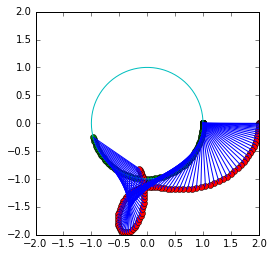
\includegraphics[width=\textwidth]{fig.png}
  \caption{Chute de la particule entre 0.0s et 2.0s}
 \end{subfigure}
 \begin{subfigure}{0.4\textwidth}
  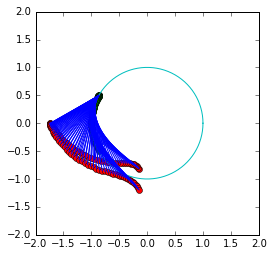
\includegraphics[width=\textwidth]{fig2.png}
  \caption{Chute de la particule entre 2.0s et 4.0s}
 \end{subfigure}
\caption{Simulation de la chute de la particule entre 0.0s et 4.0s}
\end{figure}

\pagebreak

\subsection{Disque attaché au contrepoids}

Maintenant qu'on a réussi a modéliser le mouvement d'une particule attachée à un disque, il faudra étudier le mouvement du disque
attaché au contrepoids. On dira que ce contrepoids ($P$) est laché à une hauteur initiale $h_0$ sans vitesse initiale et que la corde
qui attache le disque au contrepoids (et passe par une poulie) a une longueur $\ell_{P}$. On a donc,
\begin{center}
\begin{tikzpicture}
 \draw (0,0) circle (2);
 \draw (45:2) -- (45:3.5);
 \draw (52:2.75) node {$\ell$};
 \draw (58:1.3) node {$\ell_A$};
 \draw[dotted] (0:0) -- (45:2);
 \draw (45:4) circle (0.5);
 \draw (45:4) ++(-90:0.5) -- ++(-90:1);
 \draw (45:4) ++(-90:1.5) node {$\bullet$};
 \draw (45:4) ++(-90:1.5) node[below] {$P$};
 \draw[->] (0,-3) -- (0,4);
 \draw[->] (-3,0) -- (4,0);
 \draw[<->][ultra thin] (1:3.1) -- ++(90:1.3);
 \draw[<->][ultra thin] (1:3.6) -- ++(90:2); 
 \draw (0:3.1) ++(90:0.7) node[right] {$h$};
 \draw (0:3.6) ++(90:1.2) node[right] {$h_0$};
 \draw[->] (-90:0.7) arc (-90:90:0.7);
 \draw[->] (-90:1.5) arc (-90:45:1.5);
 \draw (-35:0.8) node[above left] {$\alpha_0$};
 \draw (-27.5:1.5) node[above left] {$\alpha$};
\end{tikzpicture}
\end{center}

D'où on déduit que,

\begin{align*}
 \Delta_h &= \ell_A(\alpha_0-\alpha) \\
 h_0 - h &= \ell_A(\alpha_0-\alpha) \\
 h &= h_0 - \ell_A(\alpha_0-\alpha)
\end{align*}

Autrement dit,

\begin{equation}
 y = h_0 - \ell_A(\alpha_0-\alpha)
\end{equation}

D'où

$$ \dot{y} = \ell_A\dot{\alpha}$$

Comme cette situation est superposé à la situation étudiée précedemment, l'énergie cinétique, potentielle et le lagrangien seront
ressemblables. On définit donc $T'$ tel que l'énergie cinétique du système $T = T_0 + T'$ où $T_0$ est l'énergie cinétique
dans la situation précedante et $T'$ est l'énergie cinétique issue de $P$. De même pour $V'$ et $L'$.

On a:

\begin{align*}
 T' &= \frac12m_Pv_P^2 \\
    &= \frac12m_P\ell_A^2\dot{\alpha}^2 \\
 V' &= m_Pg\left(h_0-\ell_A(\alpha_0-\alpha)\right) \\
 L' &= \frac12m_P\ell_A^2\dot{\alpha}^2 - m_Pg\left(h_0-\ell_A(\alpha_0-\alpha)\right)
\end{align*}

On en déduit,

\begin{align*}
 \frac{\partial L'}{\partial \alpha} &= m_Pg\ell_A \\
 \frac{\partial L'}{\partial \dot{\alpha}} &= m_P\ell_A^2\dot{\alpha} \\
 \frac{d}{dt}\left(\frac{\partial L'}{\dot{\alpha}}\right) &= m_P\ell_A^2\ddot{\alpha} 
\end{align*}

On introduit ces résultats dans l'équation $(3)$,

\begin{align}
  \left(\frac{I}{m_B}+\ell_A^2+\frac{m_P}{m_B}\ell_A^2\right)\ddot{\alpha} + \ell_A\ell_B\ddot{\beta}\cos{(\alpha-\beta)} &= -\frac{m_P}{m_B}\ell_A\left(\ell_A\dot{\alpha} + g\right)-g\ell_A\sin{\alpha}-\ell_A\ell_B\dot{\beta}^2\sin{(\alpha-\beta)}
\end{align}

En utilisant cette expression, on actualise les matrices, on a donc que

\begin{align*}
 A = \frac{I}{m_B}+\ell_A^2+\frac{m_P}{m_B}\ell_A^2 && E = -\frac{m_P}{m_B}\ell_A\left(\ell_A\dot{\alpha} + g\right)-g\ell_A\sin{\alpha}-\ell_A\ell_B\dot{\beta}^2\sin{(\alpha-\beta)}
\end{align*}


On calcule le nouveau déterminant $\Delta$,

\begin{align*}
 \Delta &= \left(\frac{I}{m_B}+\ell_A^2+\frac{m_P}{m_B}\ell_A^2\right)\ell_B^2 -\ell_A^2\ell_B^2\cos^2{(\alpha-\beta)} \\
	&= \left(\frac{I}{m_B}+\ell_A^2\sin^2{(\alpha-\beta)}+\ell_A^2\frac{m_P}{m_B}\right)\ell_B^2
\end{align*}

À nouveau on observe que $\Delta \neq 0$.

Donc, on n'a qu'a changer la valeur de $A$, de $E$ et du déterminant.

\begin{figure}[h]
\centering
\begin{subfigure}{0.4\textwidth}
 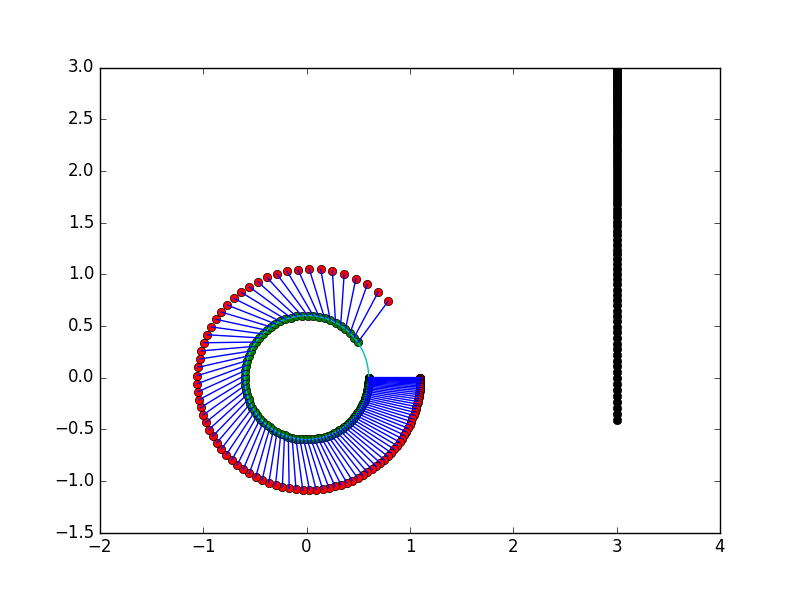
\includegraphics[width=\textwidth]{figure_3.png}
 \caption{Simulation pour $\ell_A \approx \ell_B$}
\end{subfigure}
\begin{subfigure}{0.4\textwidth}
 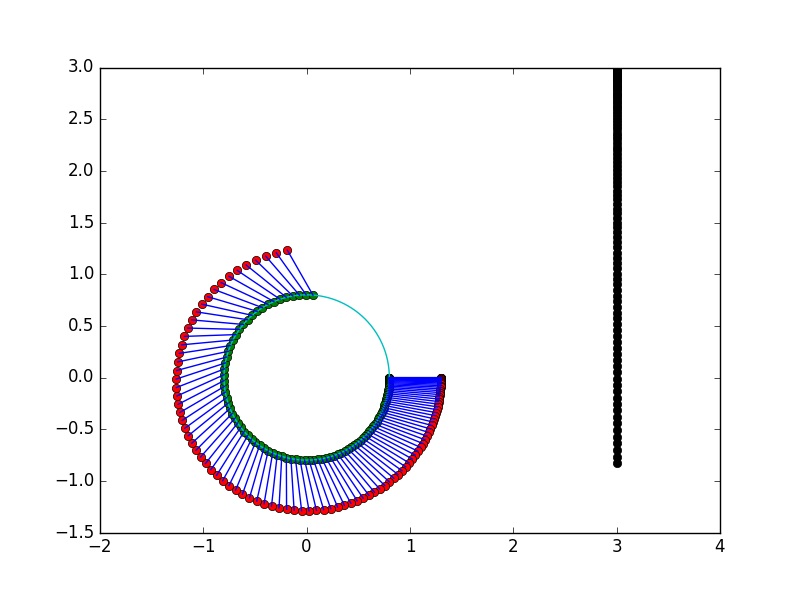
\includegraphics[width=\textwidth]{figure_4.png}
 \caption{Simulation pour $\ell_A > \ell_B$}
\end{subfigure}
\caption{Simulation pour différentes valeurs de $\ell_A$}
\end{figure}
En utilisant l'expression de la vitesse du projectile en $(1)$ et $(2)$, on détermine la vitesse à chaque instant et on obtient,

\begin{figure}[h]
\centering
  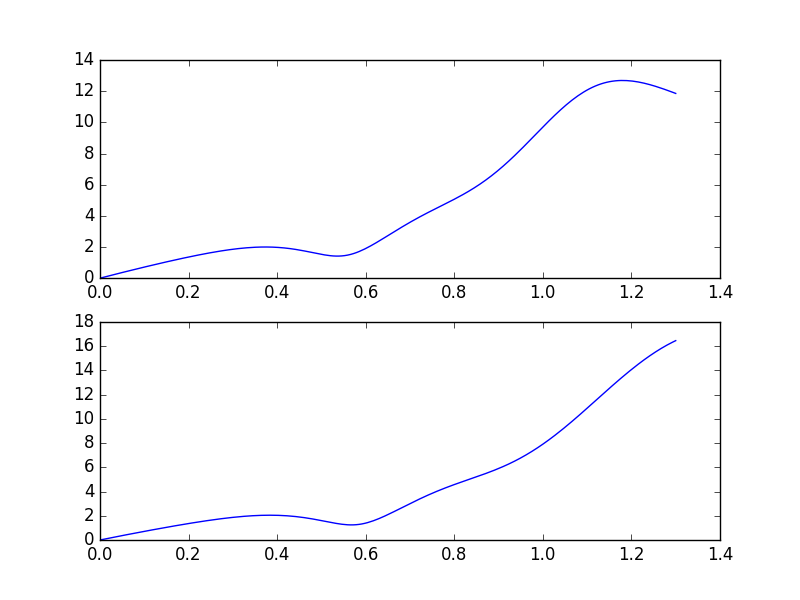
\includegraphics[width=0.7\textwidth]{figure_5.png}
  \caption{Vitesse pour $\ell_A \approx \ell_B$ et $\ell_A > \ell_B$, respectivement}
\end{figure}

\end{document}